% 2006 年上海春季卷第 21 题：原卷留白坐标网格。
% 单位网格覆盖 [-10,10]×[-10,10]，坐标轴数字按原卷显示到偶数刻度。
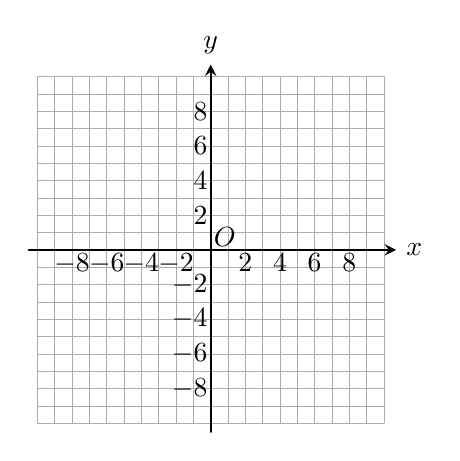
\begin{tikzpicture}[line cap=round,line join=round,x=0.22cm,y=0.22cm,>=stealth]
  \draw[step=1,gray!65,very thin] (-10,-10) grid (10,10);
  \draw[->,thick] (-10.5,0)--(10.7,0) node[right] {$x$};
  \draw[->,thick] (0,-10.5)--(0,10.7) node[above] {$y$};

  \foreach \x in {-8,-6,-4,-2,2,4,6,8}
    \node[below,inner sep=1pt] at (\x,0) {$\x$};
  \foreach \y in {-8,-6,-4,-2,2,4,6,8}
    \node[left,inner sep=1pt] at (0,\y) {$\y$};
  \node[above right,inner sep=1pt] at (0,0) {$O$};
\end{tikzpicture}
